\documentclass[twocolumn, traditabstract]{aa}  

\usepackage{fixltx2e}
\usepackage[english]{babel}
\usepackage{graphicx,amsmath}
\usepackage{epstopdf}
\usepackage{epsf,color}
\usepackage[mathscr]{eucal}
\usepackage{amsmath}
\usepackage{amssymb,amsfonts}
\usepackage{natbib}
\usepackage{txfonts}
\usepackage{dsfont}
\definecolor{Mygreen}{rgb}{0.00, 0.72, 0.0}
\definecolor{Mypink}{rgb}{1.0, 0.0, 0.5}
\usepackage[breaklinks, citecolor=blue, linkcolor=Mygreen, urlcolor=Mypink, colorlinks=true, debug, baseurl=' ']{hyperref}
\usepackage{float}
\usepackage{color}
\usepackage{scrextend}
\usepackage{nccmath}
\usepackage{mathtools, cuted}
\usepackage{lscape}
%\usepackage{widetext}
\usepackage{flushend}
\usepackage[T1]{fontenc}
\usepackage{gensymb}
\usepackage{diagbox}



\newcommand{\nika}{{\it NIKA}}
\newcommand{\nikad}{{\it NIKA2}}
\newcommand{\Q}{\mathcal{Q}}
\newcommand{\I}{\mathcal{I}}
\newcommand{\U}{$U$}
\newcommand{\di}{d\mathcal{I}}
\newcommand{\dq}{d\mathcal{Q}}
\newcommand{\eps}{$\varepsilon$}
\newcommand{\epsCMB}{$\varepsilon_{CMB}$}
\newcommand{\epsDET}{$\varepsilon_{det}$}
\newcommand{\rf}{$Rfd\mathcal{I}d\mathcal{Q}$}
\newcommand{\cf}{{\it Cf}}
\newcommand{\todo}[1]{\textcolor{red}{\textbf{#1}}}
\newcommand{\planck}{{\it P\small{LANCK}}}
\newcommand{\healpix}{{\it HEALPix}}
\newcommand{\spice}{{\it SPICE}}
\newcommand{\methodu}{{\it Method~1}}
\newcommand{\methodd}{{\it Method~2}}


\def\simlt{\lower.5ex\hbox{$\; \buildrel < \over \sim \;$}}
\def\simgt{\lower.5ex\hbox{$\; \buildrel > \over \sim \;$}}
\def\NIKA{\textit{NIKA}}

\bibpunct{(}{)}{;}{a}{}{,}
\bibliographystyle{aa}

\begin{document}
\title{KID systematics and CMB polarization blabla}
\author{A.~Andrianasolo \inst{\ref{IPAG}}\thanks{Corresponding author:
  Aina Andrianasolo, \url{aina.andrianasolo@univ-grenoble-alpes.fr}}
\and  N.~Ponthieu \inst{\ref{IPAG}}
\and  F.-X.~D\'esert \inst{\ref{IPAG}}
\and  M.~Calvo \inst{\ref{Neel}}}

\institute{
Univ. Grenoble Alpes, CNRS, IPAG, F-38000 Grenoble, France 
  \label{IPAG}
    \and
Institut N\'eel, CNRS and Universit\'e Grenoble Alpes, France
  \label{Neel}
}


\date{Received \today \ / Accepted --}
	
\abstract{Here goes the abstract}
\titlerunning{KIDs systematics}
\authorrunning{TBD}
\keywords{Techniques: polarization -- KIDs --  individual: NIKA }
\tableofcontents
\maketitle


\section{Introduction}
\label{sec:introduction}

%Pour citer les papiers: \citep{planck2013mission} ou alors
%\citep{2010A&A...518L.100M,arzoumianian}.


%\begin{itemize}
%\item Why we want to measure CMB polarization B modes
%\item The need for matrices and the KID solution, quickly mention other
%  solutions and multiplexing
%\item Importance to master systematic effects (ref. to previous papers)
%\item KIDs are a new technology that has not yet reached a ``space proof''
%  maturity. In this paper, we address a few specific systematics to KIDs.
%\item Outline
%\end{itemize}


Precise measurement of the cosmic microwave background (CMB) predicted by the $\Lambda$CDM model is one of the major challenges in cosmology. In fact, the CMB anisotropies represent an essential source of information on the physics of the early Universe as it will help us determine the origin of large scales structure and constrain the cosmological parameters of the $\Lambda$CDM model. Since the discovery of the CMB (PENZIAS), several experiments, COBE \citep{1992ApJ...396L...1S}, WMAP \citep{2013ApJS..208...20B}, Planck \citep{2016A&A...594A...1P}, have made precise measurement of CMB temperature anisotropies. These detections have permitted to support the predictions of the $\Lambda$CDM model concerning the primordial nucleosynthesis, formation of structure and on inflation, however these measurements alone can not determine all of the cosmological parameters. The next objectif for the CMB community is the measurement of the CMB polarization and in particular the detection of $B$ modes polarization. The key motivation for CMB polarization measurements is that  inflation models predict the generation of a gravitational wave background. It has been shown that a primordial gravitational wave background would leave an imprint on the polarization pattern of the CMB in the form of B mode polarization \citep{1997PhRvD..55.1830Z, 1997PhRvD..55.7368K}. The measurement of B mode polarization induced by primordial gravitational wave would then provide a powerful probe of inflation. The level of B modes is characterized by the tensor-to-scalar ratio, $r$. The current upper limit on $r$ is < 0.07 ($95 \%$ confidence) \citep{2016PhRvL.116c1302B}. Several missions focused on the detection of B modes, such as LiteBIRD \citep{2014JLTP..176..733M} or COrE \citep{2011arXiv1102.2181T}, are proposed with the objectif of having a sensitivity to be able to detect B modes at the level of $r \sim 10^{-3}$. The level of B mode polarization is several order of magnitude below the level of temperature fluctuations and polarized foregrounds, consequently, B modes can easily be degraded by various systematic effect due for exemple to temperature to polarization leakage. Together with high sensitivity, an instrument aiming at measuring the B modes requires a strict control of systematic effects.  
Some of these effects can be reduced in the design of the instruments while others have to be simulated and corrected a posteriori. Numerous systematic effects arise from optical and instrumental imperfections, temperature drifts of the optics and detectors, coupling between instrument imperfections and astrophysical foregrounds and the detector non-linearity. These effects can be modelled and characterized by the spurious signal $C_{l}$ they produce \citep{2008PhRvD..77h3003S,quickpol}. \\
The faintness of B modes signal requires the need to study the Universe at high sensitivity. To do so, the development of large detector arrays is required. Most of the detectors currently used are bolometers such as Transition Edge Sensors (TES), they are installed on experiments such as POLARBEAR \citep{2014ApJ...794..171P} or EPIC \citep{2008arXiv0805.4207B}. Performances of current bolometers are reaching the CMB photon noise limit. The need to build large detector arrays necessitate the development of detectors adapted to strong frequency domain multiplexing. In this context, TES are limited and a new kind of detectors was developed : the Kinetic Inductance Detectors (KIDs), proposed by \citet{2003Natur.425..817D}. Since 2007, these detectors have been developed for the construction of NIKA2 and its prototype NIKA (New IRAM Kids Arrays), which is the first operational instrument using KIDs \citep{2010A&A...521A..29M,2016JLTP..184..816C}. The main characteristic that makes KIDs one of the best candidates to large size detector array is their natural multiplexing capability. Indeed, the resonant frequencies of a resonator can be easily controlled during the array design, and the sharpness of the resonances allows many resonators to be placed into a limited bandwidth. Thus, a large number of resonators, can be coupled to a single transmission line, each one resonating at a different frequency $f_{0}^{i}$ \citep{2010A&A...521A..29M,Calvo2008}.\\
In this paper, we adress specifically the issue of non-linearity. This issue has so far not been addressed in the literature and is of particular relevance to the way KIDs are read out. Many polarization experiments such as  \emph{POLARBEAR} \citep{2017JCAP...05..008T} and \nika2 \citep{2017A&A...599A..34R} use a half wave plate (HWP) to improve the sensitivity in polarizatioon measurements, however the modulation of the HWP induces a strong parasitic signal that is several order of magnitude higher than the noise level. In this paper we will also adress the question of non-linearity that can be brought by this parasitic signal. These issues complement the list of specifications that must be put in instrumental designs in view of a space mission.\\
The paper is organized as follows: Sect.~\ref{sec:cmb} presents the impact of non-linearity on CMB polarization measurements, Sect.~\ref{se:kids} presents a description of physical properties of KIDs and their photometry, Sect.~\ref{se:KID_NL} shows the impact of KID non-linearity on observations and Sect.~\ref{se:scan_strat}


\section{Measurement of the CMB...}

\subsection{Introduction of the problem and main equations}
\begin{itemize}
\item equations pour montrer l'impact de la non linearite
\item plot qui montre le niveau de NL tolerable sur du CMB pur (les Cl actuels)
  et le niveau de residus de foregrounds qu'on peut tolerer aussi (TE, EB,
  TB...)
\item Careful with the actual (single sky) correlation between foregrounds and
  CMB that does not cancel ou ``on stat average''...
\end{itemize}

\subsection{Simulations}
\subsubsection{CMB NL residuals}

\subsubsection{Foregrounds residuals}

\begin{itemize}
\item compute foregrounds' alms (polarized) and propagate to power spectra =>
  take 353GHz dust polarized map and 30GHz (which is best) synchrotron
  template. Warning: ringing vs large scale domination
\end{itemize}


\section{Kinetic Inductance Detectors}
\label{se:kids}


%\subsection{Presentation rapide des detecteurs}
%\subsection{Photometrie}
%\subsubsection{Rf}
%\subsubsection{Cf}
%
%\subsection{Non linearite par l'observation d'une source ponctuelle}

%%%%

\subsection{Description}

The theory of superconductivity described by \citep{PhysRev.108.1175} show that at low temperature, there is an attraction between electrons due to electron-phonon interactions that bind electrons together to form call Cooper pairs \citep{PhysRev.104.1189}. In superconductors this state is primarily responsible for superconductivity. When incident photons with sufficient energy are absorbed by the detector's superconducting film, they break Cooper pairs which increases the quasi-particles density and causes a change in the kinetic inductance $L_{K}$. The shift in the kinetic inductance $\delta L_{K}$ is proportional to the density of quasi-particles $\delta L_{K} \propto \delta n_{qp}$, which is directly proportional to the absorbed incident power : $\delta n_{qp} \propto \delta P_{opt}$.
Kinetic Inductance Detectors (KIDs) are RLC superconducting resonator introduced by \citep{2003Natur.425..817D} and that use this principle. Their resonant frequency is given by : 

\begin{equation}
f_{0} = \frac{1}{2\pi \sqrt{(L_{k}+L_{G})C(\varepsilon)}}, 
\end{equation}
 
where $L_{K}, L_{G}$ and $C$ are the resonator's kinetic inductance, geometric inductance and capacity. $\varepsilon$ is the material permittivity.
When a KID absorbs photons, its resonant frequency varies like :

\begin{equation}
\delta f_{0} = -\frac{1}{2}C(\varepsilon)f_{0}^{3} \delta L_{K}.
\end{equation}

A small change in the kinetic inductance results in a proportional shift of the resonant frequency. As a result, there is a linear relation between the absorbed optical power by the detector and the shift of the resonant frequency :

\begin{equation}
\delta f_{0} \propto -\delta P_{opt}.
\end{equation}

This is represented in Fig.~\ref{fig:resonance}. It is then possible to measure a variation of flux on the sky by measuring the shift of resonant frequency of a detector. Two methods that are use to follow this shift are described further.

\begin{figure}
  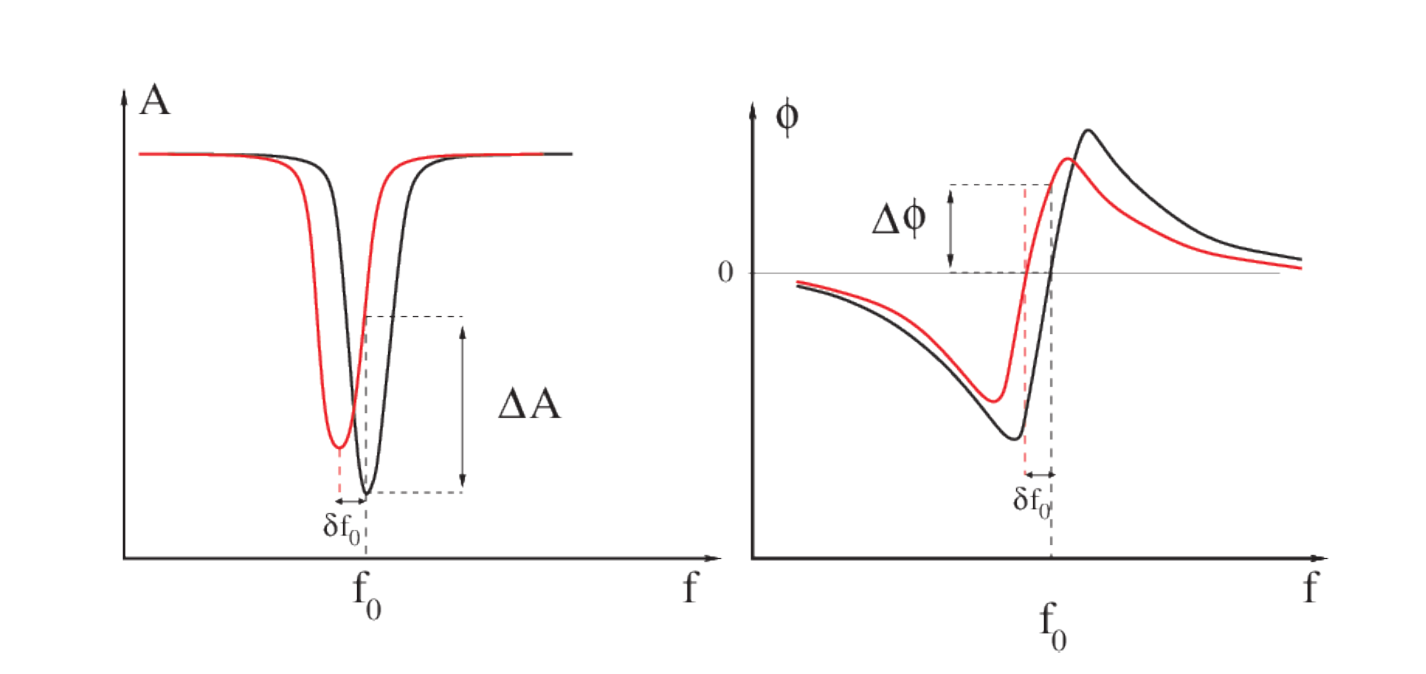
\includegraphics[clip, angle=0, width=\columnwidth]{Figures/resonance.png}
  %	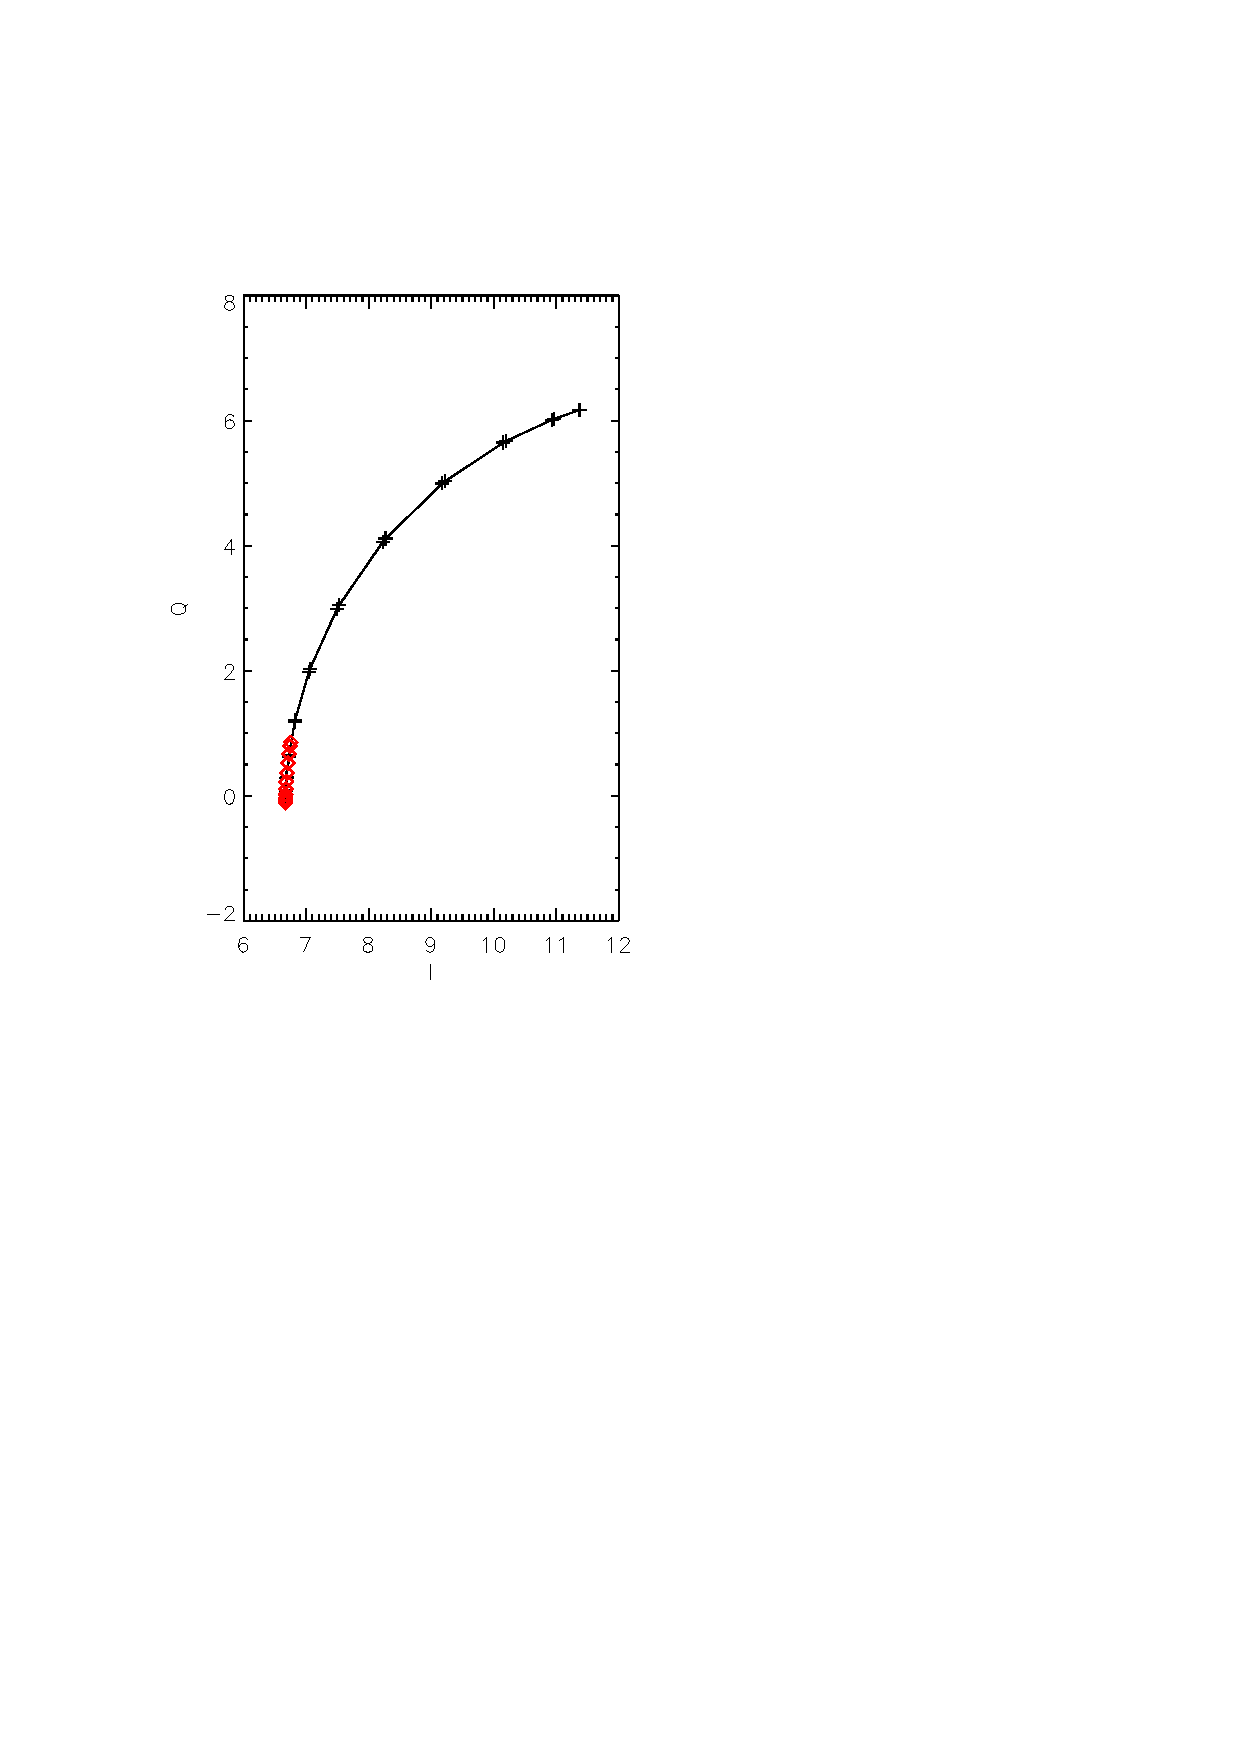
\includegraphics[clip, angle=0, width=\columnwidth]{Figures/resonance.pdf}
  \caption{Schematic representation of a KID resonance in amplitude (left) and phase (right), as a function of the excited tone injected in the feedline. The optical power absorbed by the detector is weak for black curves and increases for red curves. The absorption of a photon shifts the resonance frequency and this is directly proportional to the received power.}
  \label{fig:resonance}
\end{figure}


\begin{figure}
\center
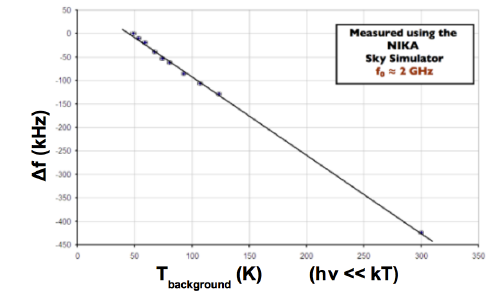
\includegraphics[clip, angle=0, width=\columnwidth]{Figures/KID-linearity-Monfardini2014.png}
\caption{KID linearity demonstrated in laboratory under realistic
  conditions. The plot shows the frequency shift of the resonance as a function
  of the optical background temperature (K). Solid line : linear fit of the
  experimental points. Credits : \citet{2014JLTP..176..787M}.}
\label{fig:KID-lin}
\end{figure}

Laboratory measurements with \todo{XXXX describe set up XXX} have shown that
KIDs are linear over a wide range of backgrounds (Fig.~\ref{fig:KID-lin}). Like all detectors, measures done by KIDs can become non-linear at a certain point. Physically, non-linearity in a KID could appear as a consequence of too strong currents inside the resonator or to too strong induced magnetic fields. This leads to an increase in the quasi-particles density and the kinetic inductance, which could cause a loss of superconductivity \citep{Calvo2008} \todo{(articles Pippard, Parmenter ?)}. In this paper, we will study KID non-linearity in different conditions. 

%Kinetic Inductance Detectors (KIDs) are RLC superconducting resonator, made from a thin metal film and introduced by \citep{2003Natur.425..817D}. They are based on a novel superconducting detector technology that provides high sensitivity and ease of multiplexing. 
%
%\citep{2016A&A...592A..26C} show that KID arrays behave appropriately in a space-like environment, they present short time constants making them less sensitive to cosmic rays compared to bolometers. This features make KIDs competitive with other technologies to be implemented in futur ground base or space CMB mission.
%In this section we give a brief summary of their main features and how photometry can be derived from their measurements, then we study the KID non-linearity, a systematic effect that must be taken into account in the design of futur experiments.
%
%This relation is linear for small variations in $P_{opt}$
%\citep{2010ApPhL..96z3511S}. 

\subsection{Transfer function}

A KID circuit is coupled to a transmission feedline that is expressed by the $S_{21}$ parameter. The KID transfer function reads : 

\begin{equation}
S_{21}(f) = \mathcal{I} +j\mathcal{Q} .
\end{equation}

\noindent where $\mathcal{I}$ and $\mathcal{Q}$ give respectively the real (in phase) and imaginary
(quadrature) of $S_{21}$. A model of a KID transfer function has been proposed
by \citet{2008ApPhL..93m4102G} :

\begin{equation}
S_{21} = \frac{2Z_{res}Z_{0}}{Z_{res}[2Z_{0} + j(X_{1}+X_{2})] + (Z_{0} +jX_{1})(Z_{0} +jX_{2})},
\end{equation}

with:

\begin{equation}
Z_{res} = \frac{Z_{0}Q_{e}}{2Q_{i}}[1 + 2jQ_{i}\frac{(f-f_{0})}{f_{0}}],
\end{equation}

\noindent where $X_{1}$, $X_{2}$, $Z_{0}$ are impedances, $Q_{i}$ is the
intrinsic quality factor of the resonator and $Q_{e}$ is the external quality
factor due to coupling with the measurement electronics. $f$ is the frequency of
excitation of the detector, and $f_{0}$ is the resonant frequency. Throughout
this paper, we shall assume typical values of KIDs $X_{1} = X_{2} =
0.5\,\Omega$, $Z_{0} = 50\,\Omega$, $Q_i=2\times 10^4$, $Q_e=10^4$ and $f_{0} =
1.8\times 10^9$\,Hz as measured on \nika\ and \nikad. The following section
addresses how the resonance of a KID is monitored and related to the incident
optical power.

% \section{Methods of signal reconstruction}
\subsection{Photometry}
\label{sec:signal}

A dedicated KID readout system has been developed by \citet{2013A&A...551L..12C}
and successfully used for \nika\ and \nika2\ \citep{2010A&A...521A..29M,2016JLTP..184..816C}. We here summarize its main charcteristics and the observables
that are relevant for our simulation work. We then present two ways to use them
to derive the photometry.

%% To convert the $\I(t)$ and $\Q(t)$ that
%% describe the resonance frequency shift $\delta f_0$ to the absorbed optical
%% power $\delta P_{opt}$. We have devised two ways to relate these
%% quantities. Both rely on a specific electronic modulation readout devised by
%% \citet{2013A&A...551L..12C} that we summarize first.

\subsubsection{Modulated readout technique}

\begin{figure}
  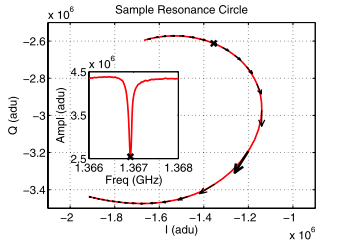
\includegraphics[clip,angle=0,width=\columnwidth]{Figures/resonance-circle.png}
  \caption{Trajectory of $\I$ and $\Q$ during a frequency sweep around the
    resonance of a KID. The arrows represent $(\di,
    \dq)$. \citep{2013A&A...551L..12C}}
  \label{circle-iq}
\end{figure}

The excitation tone frequency of a KID is modulated by a local oscillator with a
known frequency shift. This provides two values $f_{\pm} = f_0 \pm \delta
  f_{LO}/2$ with $\delta f_{LO} \simeq 1$\,kHz. Time ordered data values $(\mathcal{I}(t),\mathcal{Q}(t))$ are given by :

\begin{equation}
(\mathcal{I}(t), \mathcal{Q}(t)) = (\frac{\mathcal{I}(f_{+}) +
    \mathcal{I}(f_{-})}{2},
\frac{\mathcal{Q}(f_{+}) + \mathcal{Q}(f_{-})}{2}),
\end{equation}

and the differential values are :

\begin{equation}
\label{gradient}
(\frac{\di}{df}(t), \frac{\dq}{df}(t)) =
\left(\frac{\I(f_{+}) - \I(f_{-})}{\delta f_{LO}},
\frac{\Q(f_{+}) - \Q(f_{-})}{\delta f_{LO}}\right).
\end{equation}

These quantities are represented on Fig. \ref{circle-iq}. In this paper, we take
typical laboratory values and assume that $i$ and $q$ are sampled at
880\,Hz. This high acquisition rate is allowed by the sub-millisecond time
constant of the KIDs. For most experiments, such a high sampling rate is not
required and we average these measures over 40~samples to produce
four secondary quantities at 22\,Hz:

\begin{eqnarray}
\I  &=& \sum^{N_{m}=40}_{p=1} i_{p},\\
\Q  &=& \sum^{N_{m}=40}_{p=1} q_{p},\\
d\I &=& \sum^{N_{m}/2=20}_{p=1} i_{2p} - i_{2p-1},\\
d\Q &=& \sum^{N_{m}/2=20}_{p=1} q_{2p} - q_{2p-1}.
\end{eqnarray}

With these quantities in hand we have two methods to derive the transmitted
signal. They are presented in the following paragraphs.

\subsubsection{\methodu}
If a variation $\Delta\I(t)$, $\Delta\Q(t)$ is observed between successive ($\I$,
$\Q$) points, it is possible to estimate the shift of the resonant frequency
$\Delta f_{0}$ between these two samples by comparing ($\Delta \I$, $\Delta \Q$)
with the gradient $(\di,\dq)$ induced by the known and small $\delta
f_{0}$ of the local oscillator. This is done by a scalar projection of ($\Delta\I$,
$\Delta\Q$) on $(\di,\dq)$ that is tangent to the resonance circle. To have a
cleaner estimation of the latter, we take its running average over 50
points that we write $\langle . \rangle_{50}$ \citep{2014A&A...569A...9C}:

\begin{equation}
\label{eq:Rf}
\Delta f_{0} = \delta f_{LO} \frac{\Delta \I\, \langle \di
  \rangle_{50}
+ \Delta \Q\, \langle \dq \rangle_{50}}{\langle \di
  \rangle_{50}^{2}
 + \langle \dq \rangle_{50}^{2}},
\end{equation}

Note that this average is performed only on the tangent vector $(\di,\dq)$ so
that $\Delta f_0$ is sampled like $\I$ and $\Q$ at 22\,Hz. This method has been
successfully used in \nika\ and \nika2. Under large incoming power, the resonances can be shifted far from their excitation frequency. The $(\I, \Q)$ circle is then distorted and the tangent approximation of $(\di, \dq)$ no longer holds which can be the source of non-linearity. In the next paragraph we present an improved method to follow the shift of the resonant frequency.

\subsubsection{\methodd}

\begin{figure}
\includegraphics[clip, angle=0, width=\columnwidth]{Figures/circle_zres.eps}
\caption{Bottom: location of $\I$ and $\Q$ when a KID observes a point source of
  various fluxes. Top: ratio of the distance between $(\I,\Q)$ and the center of
  the fitted circle over the radius of this circle. All the points on the pure
  imaginary line at $\I=1$ are the result of the transformation of the circle
  into $Z_{res}$ according to eqs.~(\ref{eq:z_res}) and
  (\ref{eq:scale_rotate}).}
\label{fig:circle_zres}
\end{figure}

\todo{ref to the circular nature of (I,Q): \cite{2011ApJS..194...24M}}.\\

To improve \methodu, we developed a new technique that fully exploits the circular
nature of the $(\I,\Q)$ trajectory, hereafter called \methodd. It is
  based on the transformation property of a circle in the complex plane into a
  straight line. Indeed, let us consider a circle centered on $(0,1/2)$ with a
  radius of $1/2$ and compute its inverse:

\begin{eqnarray}
Z_{ref} &\equiv&\frac{1}{2} + \frac{1}{2}e^{i\phi}\,, \\
&=&\cos\frac{\phi}{2}e^{i\phi/2}\,,\\
Z_{res} &\equiv& 1/Z_{ref}\,, \label{eq:z_res} \\
&=&1-i\tan\frac{\phi}{2}\,.
\label{eq:z_res}
\end{eqnarray}

$Z_{res}$ is a straight line and along this line $Z$ varies linearly with
$\phi$ for small values of $\phi$. Experimentally, we are in this regime
when the signal is weak and when $\phi$ is defined w.r.t.~ the $(O,C)$ axis
as defined on Fig.~\ref{fig:circle_zres}. We thus fit the radius $r$ and the
center $(\I_c,\Q_c)$ of our measurement circle $Z=\I+j\Q$. Defining
$\alpha=\arctan\Q_c/\I_c$, we scale, rotate and translate this
circle to the $Z_{res}$ circle according to

\begin{equation}
Z_{ref} = \left(\begin{array}{c}
\I_{ref}\\
\Q_{ref}\end{array}\right) = 
\frac{-1}{2r}\left(\begin{array}{rr}
\cos\alpha & \sin\alpha\\
-\sin\alpha & \cos\alpha\end{array}\right)
\left(\begin{array}{c}
\I-\I_c\\
\Q-\Q_c\end{array}\right) +
\left(\begin{array}{c}
1/2\\
0\end{array}\right)
\label{eq:scale_rotate}
\end{equation}

The result of this transformation is shown on Fig.~\ref{fig:circle_zres}. A
variation of the signal $(\Delta\I,\Delta\Q)$ leads to a variation
$\Delta\phi$ along $Z$ that is proportional to the frequency shift $\Delta f$
that we are after to determine photometry. To derive the calibration between
these two quantities, we once again rely on the $(\di,\dq)$ that is induced by
the known $\delta f_{LO}$. Applying transformation (\ref{eq:scale_rotate}) to
$(\di,\dq)$, we obtain the corresponding variation $dy = Im(dZ_{res})$. The
final derivation of $\Delta f$ corresponding to $(\Delta\I,\Delta\Q)$ requires
the integration of $dy/\delta f_{LO}$. For the sake of simplicity, we fit
$Im(dZ_{res})$ as a polynomial of $dy/\delta f_{LO}$ that is therefore trivial
to integrate.\\

%% \begin{equation}
%% \tan\frac{\delta\phi}{2} \simeq \frac{\delta\phi}{2} +
%% \frac{(\delta\phi)^3}{15}
%% \end{equation}


In addition to the non-linearity induced physically by a loss of superconductivity, non-linearity can also arise from the methods that we use to recover the incident optical power. In fact, when the source is very bright (such as planets of several tens of Jy) the change of the density of charge carriers can shift the resonances far from their excitation frequency, and lead to $(\I,\Q)$ measures that leave the resonance circle, hence invalidating the approximations made in the photometric equations of the previous section. This paper aims at showing the linearity of \methodu\ and the improvement that can be made with \methodd . Another possible source of non linearity is the instrument scanning speed. Indeed, even if the source is moderately bright, if it is scanned too fast, $(\Delta\I,\Delta\Q)$ could be far from the tangent vector $(\di,\dq)$ which would alter their linear relation.
In this paper we study the impact of non-linearity of a KID on the measure of B modes. In the next section, in a first part we study the impact of non-linearity in total power. In a second part we study the impact of non-linearity induced in polarization measurements by a rotating Half Wave Plate (HWP).

%Induced non-linearities in the two last cases result in a poor reconstruction of the shift of the resonant frequency. In principle this problem should be improved with the \methodd\ method. In this paragraph, we explore the two last cases.\\

\section{Impact of KID non-linearity}
\label{se:KID_NL}

\subsection{Total power}

In this paragraph we characterize KID non-linearity in total power. To do so, we simulate the observation of a point source by a KID, with a flux that we vary between \todo{1 and 2000\,Jy TBC} (fluxes are unrealistically large on purpose for illustration), to see how linear the measure remains. We assume that our instrument has a 11\,arcsec FWHM Gaussian beam like the polarized 1\,mm channel of \nikad. In the simulation, we use \methodu\ and  \methodd\ to recover the received power. We write the non linear detector response as :

\begin{equation}
m = m + \varepsilon_{det} m^2 +c_{0}.
\label{eq:model_kid_nl}
\end{equation}

\epsDET\ represents the non linearity of the KID. 
For all simulations we compute the non-linearity coefficient \epsDET\ from eq.~(\ref{eq:model_kid_nl}) by doing a linear fit of the input fluxes as a fonction of output fluxes.

Fig.~\ref{fig:planet_profiles} and Fig.~\ref{fig:flux_out_vs_in} show that under a bright source, non-linearity appears with the distortion of the input gaussian profile in the case of \methodu\ whereas \methodd\ remains linear on the same flux scale. The non-linearity coefficients that we find with \methodu\ and \methodd\ are respectively \epsDET =$-2.22 \times 10^{-5}$ and \epsDET =$8.69 \times 10^{-8}$. 



\begin{figure}
  \includegraphics[clip, angle=0, width=\columnwidth]{Figures/planet_profiles_2.eps}
  \caption{Comparison of an incoming flux that we vary between 1 and 2000 Jy TBC (in black), with flux reconstructed by \methodu\ and \methodd. Fluxes are unrealistically large on purpose for illustration. }
  \label{fig:planet_profiles}
\end{figure}


\begin{figure}
  \includegraphics[clip, angle=0, width=\columnwidth]{Figures/flux_out_vs_in.eps}
  \caption{Comparison of an incoming flux that we vary between 1 and 2000 Jy TBC (in black), with flux reconstructed by \methodu\ and \methodd. Fluxes are unrealistically large on purpose for illustration. }
  \label{fig:flux_out_vs_in}
\end{figure}


Simulations of a KID non-linearity in total power meets the requirements (see Sec.~\ref{cmb}) necessary to not biais measures of B modes. In CMB polarization experiments, the use of Half Wave Plate to modulate polarization are more and more considered. In the next section we will study the effect that can have this signal on the KID linearity.

%In futur CMB polarization experiments, the use of a half wave plate more and more common. It presents a lot of advantages, but can also be source of various systematic effects. In the next section we will address the non-linearity that can arise from rotating a half wave plate in an instrument.

%KIDs are a novel technology successfully used in \nikad . Because of their multiplexing capability and their short time constant, they are one of the best candidates to be implemented on experiments that need larger arrays. In this section we studied KIDs non-linearity and its impact on CMB B mode measures, considering the brightness of a source, the scanning speed of the instrument and the method that we use to follow the shift of the resonant frequency and retrieve the absorbed power.
%Simulations of a KID exposed to a point source with a large variation of fluxes have shown that as expected, the brighter is the source, the more non-linearities appear due to a poor reconstruction of the resonant frequency. Although both reconstruction methods give good results, \methodd\ remains more linear at high fluxes than \methodu . Plus, KID non-linearity should not impact measures of CMB B modes, in fact the non-linearity coefficients that we found are in the range of $[10^{-5} - 10^{-8}]$, so it meets the requirement addressed in Sec.\ref{sec:cmb}.


\subsection{Polarization and Half Wave Plate}
\subsubsection{Half Wave Plate}

%\begin{itemize}
%\item les HWP deviennent a la mode
%\item les kids ont des constantes tres petites, donc on peut faire tourner vite
%  : avantages...
%\item ... mais signal parasite tres fort et donc besoin de le soustraire et de
%  voir si il n'induit pas de non linearite sur la mesure du signal
%\item simulations du \mathcal{H} (beta): bien expliquer que ce qui compte c'est la
%  subtraction of this template not the exact recovery of the input model
%\item which constraints do we set on the \mathcal{H} subtraction and potential
%  improvement if we could use hundreds of KIDS rather than just fit it kid by kid
%\item anticipate a bit on the achieved residual NL on the same planet as in the
%  previous section.
%\item simulate the sum of a template and pure weak signal and see the induced NL
%  on the signal
%\item comparison to NIKA(2)'s data... vs Simon's observatory perspectives
%\end{itemize}

%{\color{blue}
%Modulation of the polarization by a rotating Half Wave Plate (HWP) like in
%\nika\ and \nikad\ creates a background modulation equivalent to several tens to
%hundreds of Jy at frequencies close to the HWP rotation harmonics
%\citep{2017A&A...599A..34R}. After early tests by \todo{cite Hildebrand in the
%  80's or so ?}, this kind of modulating device has been left aside for
%\todo{20~TBC} years in the context of millimetric observations. With the
%improvement of technologies it progressively came back in the landscape, in
%particular with pioneering experiments like \emph{Maxipol}
%\citep{2007ApJ...665...42J} and \emph{EBEX} \citep{2010SPIE.7741E..1CR}. It is
%now more and more common and is considered as the leading option for future
%satellite designs such as \emph{LiteBIRD} \todo{add ref}. Such a background must
%be accounted for in the simulations.}

After early tests by \citep{1984ApJ...284L..51H}, modulation of the polarization by a rotating Half Wave Plate (HWP) has been left aside for \todo{20~TBC} years in the context of millimetric observations. With the improvement of technologies it progressively came back in the landscape, in particular with pioneering experiments like \emph{Maxipol} \citep{2007ApJ...665...42J}, \emph{SPIDER} \citep{2008SPIE.7010E..2PC}, \emph{EBEX} \citep{2010SPIE.7741E..1CR}, \emph{Polarbear} \citep{2012SPIE.8452E..1CK} \emph{BLAST-Pol} \citep{2014MNRAS.437.2772M}, \emph{ABS} \citep{2014RScI...85c9901K} and \emph{Advanced ACTPol} \citep{2016JLTP..184..772H}. It is now more and more common and is considered as the leading option for future satellite designs such as \emph{LiteBIRD} \citep{2014JLTP..176..733M} and next generation ground based experiments such as \emph{CMB-S4} \citep{2016arXiv161002743A}. The rotation of the HWP can be stepped (\emph{POLARBEAR} \citep{2014ApJ...794..171P}) or continuous  (\emph{EBEX}, \emph{ABS} and \nikad\  \citep{2015fers.confE..16R}). There exist different mechanism to rotate a HWP. For example, the HWP of \nikad\ is mounted inside a holder and coupled with a step motor, whereas \emph{EBEX} HWP is levitated with a superconducting magnetic bearing.
Using a HWP to modulate the polarization is a powerful tool to mitigate several instrumental systematics \citep{2009MNRAS.397..634B}. In fact, with a HWP :

\begin{itemize}
\item The polarized signal is modulated at 4 times the rotation frequency of the HWP and therefore is shifted at higher frequencies, isolating it from electronic noise and 1/f noise. This is valid if the rotation of the HWP is continous and fast ( HWP rotation frequency of \emph{EBEX} and \nika\ are respectively 1.235 Hz \citep{2018ApJS..239....7T} and 2.98 Hz \citep{2017A&A...599A..34R}.)

\item A single detector $k$ can measure a combination of the three Stokes parameters $I$, $Q$ and $U$ :

\begin{equation}
\label{eq:polar_measure}
m_{k}(t) = \frac{1}{2} [I + \rho [Q \cos (4 \omega t + 2 \alpha(t)) + U \sin (4 \omega t + 2 \alpha(t))]],
\end{equation}

with $\alpha$ the angle between the telescope reference frame and the local meridian on the sky and $\omega t$ is the position angle of the HWP.
This allows to do observations without having to use differencing polarization sensitive detectors and thus avoid systematic effects such as intensity to polarization leakage from mismatch of the detector beams \citep{2008PhRvD..77h3003S, 2015ApJ...814..110B}

\item We can achieve an optimal angular coverage as each pixel will be observed over a wide range of orientations. This allows to have a better angular redundancy in a single pixel to measure the Stokes parameters without having to rotate the full instrument.
\end{itemize}

On the downside, this kind of modulation can give rise to a systematic effect that is specific to instruments using a continuously rotating HWP : the Half Wave Plate Synchronuous Signal (HWPSS). In the next paragraph, we study non-linearity that are induced by this additional signal.

\subsubsection{Half Wave Plate Synchronous Signal}

\begin{figure}[h]
\center
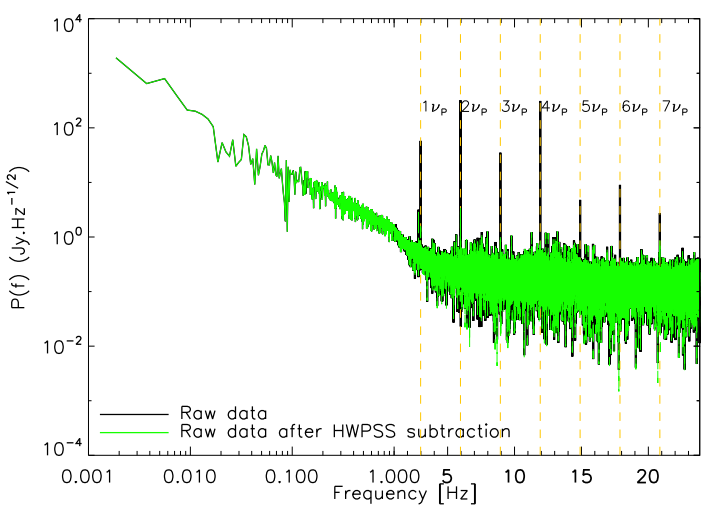
\includegraphics[clip, angle=0, width=\columnwidth]{Figures/hwp_power_spectrum.png}
\caption{Power spectrum of an observation of Orion OMC-1 for one KID. The parasitic signal is highly peaked at harmonics of the HWP rotation frequency. The observations were done with \nika . Black and green lines represent respectively the raw data and the raw data after subtraction of the HWP parasitic signal \citep{2017A&A...599A..34R}. }
\label{fig:hwp_power_spectrum}
\end{figure}

\begin{figure}[h]
\center
\includegraphics[clip, angle=0, width=\columnwidth]{Figures/hwpss_2pi.eps}
\caption{Representation of the parasitic signal as a function of angles of the HWP. The points are gathered around precise values of angles because the acquisition is synchrnous with the HWP rotation. Red dots correspond to the points reconstructed by the model of eq.~\ref{eq:hwp-template}. Blue curve corresponds to the model on one period.}
\label{fig:hwpss_2pi}
\end{figure}

Non-idealities of the HWP can create a background modulation equivalent to several tens of Jy at frequencies close to the HWP rotation harmonics \citep{2017A&A...599A..34R} (see Fig.~\ref{fig:hwp_power_spectrum} and Fig.~\ref{fig:hwpss_2pi}). This HWP synchronous signal (HWPSS) was observed by \emph{MAXIPol} \citep{2007ApJ...665...42J}, \emph{EBEX} \citep{2010SPIE.7741E..1CR}, \emph{POLARBEAR} \citep{2017JCAP...05..008T} and \nika\ \citep{2017A&A...599A..34R}, although they have different HWP and HWP rotation mechanism. This signal must be subtracted from observations or it will dominate polarization. To do that, we can model it by a sum of $n$ harmonics of the HWP rotation frequency $\nu_{p}$ with amplitudes $A_{n}$ and $B_{n}$ that are linearly drifting :

\begin{equation}
\mathcal{H}(t) = \sum_{n=1} A_{n} \cos n\omega t + B_{n} \sin n \omega t , 
\label{eq:hwp-template}
\end{equation}

where : 
\begin{eqnarray}
A_{n}  &=& A_{n}^{0} + \varepsilon_{A_{n}}t,\\
B_{n}  &=& B_{n}^{0} + \varepsilon_{B_{n}}t, 
\end{eqnarray}

with $\omega = 2 \pi \nu_{p}(t)$.
This effect can then be corrected by subtracting observations by the model presented in eq.~\ref{eq:hwp-template}. 

A large amplitude of $\mathcal{H}(t)$ could bias the measurement and the photometry by causing non-linearity in the detector response. This non-linear response can then be the source of coupling between intensity and polarization signals. Systematic effects arising from detector non-linearity have been studied in \emph{Simon's Observatory} \citep{2018SPIE10708E..48S}, \emph{POLARBEAR} \citep{2017JCAP...05..008T} and \emph{EBEX} \citep{2017arXiv171101314D}. In the latter, it was shown that the dominant source of intensity to polarization leakage is due to detector non-linearity caused by a large HWPSS \citep{2017arXiv171101314D}.

In \nikad\ this additionnal noise is two to three order of magnitude above the noise level, making it one of the strongest noise contributor in polarization observations, such a bakground must be accounted for in the simulations. In the next paragraph, we study the non-linearity of a KID caused by a large HWPSS. 

\subsubsection{Simulations}

In our simulation, we test the impact of this parasitic signal on the observations and if the residuals left by the subtraction of $\mathcal{H}$ can create non-linearity. We keep the instrumental parameters of Sect.~\ref{se:kids} and we simulate the observation of a point source, with a flux that varies between 1 and 500 Jy. To account for the parasitic signal $\mathcal{H}$, we build a template following eq.~\ref{eq:hwp-template}, with a maximum amplitude of 70 Jy as seen in \nikad , that we add to the observation. To subtract this additional signal, we fit the template $\mathcal{H}$ by using the method described in \citep{2017A&A...599A..34R}, and then subtract it to our observation. We use the same method as in Sec.~\ref{se:kids} to derive the non-linearity coefficient \epsDET . Fig.~\ref{fig:histos_epsilon_rf} and Fig.~\ref{fig:histos_epsilon_cf} show the distribution of non-linearity coefficients for different method of signal reconstruction (\methodu\ and \methodd). For one realization we vary the amplitudes $A_{n}$ and $B_{n}$ of $\mathcal{H}$.

\begin{figure}
	\includegraphics[clip, angle=0, width=\columnwidth]{Figures/histos_epsilon_rf.eps}
	\caption{Histogram of non-linearity coefficients derived with \methodu\ and scanning speed equal to 3 and 5 points per beam.}
	\label{fig:histos_epsilon_rf}
\end{figure}

\begin{figure}
	\includegraphics[clip, angle=0, width=\columnwidth]{Figures/histos_epsilon_cf.eps}
	\caption{Histogram of non-linearity coefficients derived with \methodd\ and scanning speed equal to 3 and 5 points per beam.}
	\label{fig:histos_epsilon_cf}
\end{figure}

The mean value of non-linearity coefficient derived with \methodu\ and \methodd\ are respectively \epsDET = $-2.2 \times 10^{-5}$ and \epsDET =  $-4.7 \times 10^{-7}$, this show that as precedently, \methodd\ remains more linear than \methodu\ on the same flux scale. We manage to correctly subtract the HWPSS template so that it doesn't create additional non-linearities, in fact, with both methods, the non-linearity coefficients are of the same order of magnitude with or without the additional HWPSS template. The non-linearity coefficients derived from the simulations are lower than the non-linearity coefficient required in Sect.~\ref{sec:cmb} to detect B modes without being biaised by non-linearity arising from the detector and the HWPSS. 
In these simulations, we have shown that non-linearity appears when the detector is under a bright source, leading to a poor reconstruction of the signal. In the next section, study realistic simulations by using a scanning strategy typical of a satellite to scan the Galaxy which is more complex than a planet and to ensure that its signal can be reconstructed with \methodu\ and \methodd .

%
\section{Half Wave Plate modulation}

\begin{itemize}
\item les HWP deviennent a la mode
\item les kids ont des constantes tres petites, donc on peut faire tourner vite
  : avantages...
\item ... mais signal parasite tres fort et donc besoin de le soustraire et de
  voir si il n'induit pas de non linearite sur la mesure du signal
\item simulations du HWPSS (beta): bien expliquer que ce qui compte c'est la
  subtraction of this template not the exact recovery of the input model
\item anticipate a bit on the achieved residual NL on the same planet as in the
  previous section.
\end{itemize}


\section{Scanning strategy}

\begin{itemize}
\item explain how the 4f harmonics separates from the scanning frequencies
\item derive constraints on precession, nutation and scanning speed vs HWP
  speed.
\item Number of samples per beam vs combination of kids to produce a map: one
  map is the average of N independent maps *only* if *each* KID produces a full
  map. Otherwise it's a somehow classic combination of different detectors
\end{itemize}

A key factor in the design of space experiments is the scanning strategy of the instrument, as it conditions all the observations. Here, we present different simulations of scanning strategies such as the ones used in EPIC \citep{2009arXiv0906.1188B}, and Planck \citep{2005A&A...430..363D}. \\

Fig.~\ref{fig:satellite} shows a representation of a satellite, where $\alpha$ is the angle between the spin axis and the precession axis, and $\beta$ is the angle between the optical and spin axis of the satellite.
For EPIC scanning strategy, the optical axis of the telescope is inclined by $\beta$=55$\degree$ with respect to the spin axis The spin axis is inclined by $\alpha$=45$\degree$ from the precession axis and it precesses around the Sun-Earth axis every hour.
Planck scans large circles on the sky with a 85$\degree$ angle between the optical axis and the spin axis. The precession angle is 7$\degree$.

\begin{figure}[h]
  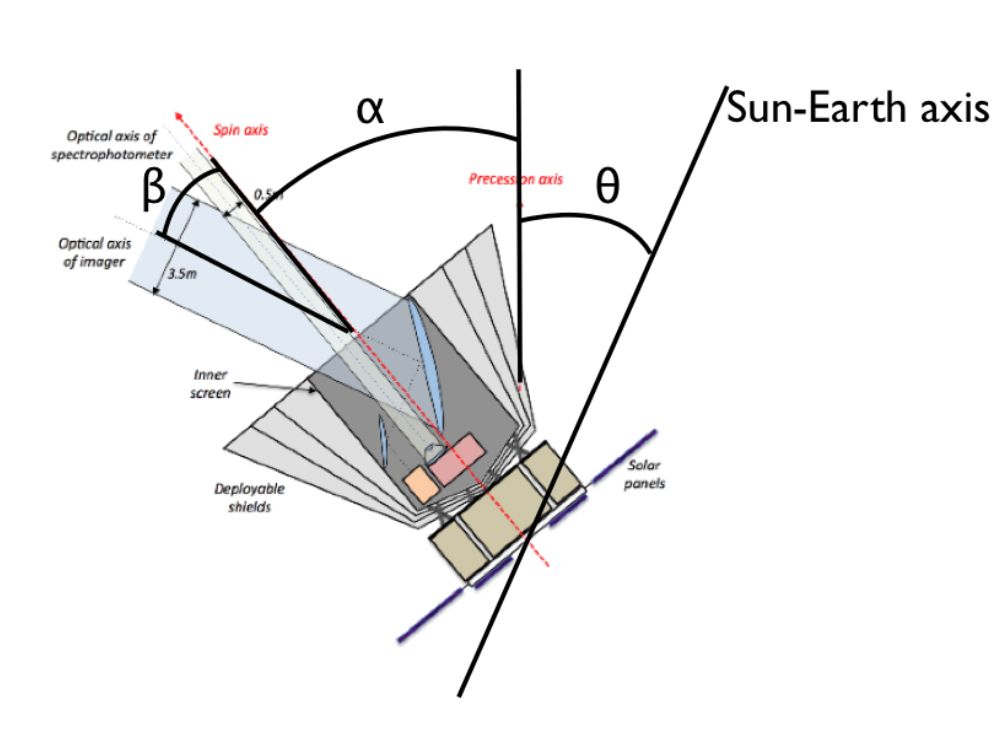
\includegraphics[clip,angle=0,width=\columnwidth]{Figures/schema_satellite.png}
  \caption{Schematic view of a satellite}
  \label{fig:satellite}
\end{figure}

The two scanning strategies are represented in Fig.~\ref{fig:strat-polsat-Planck}.

\begin{figure}[h]
  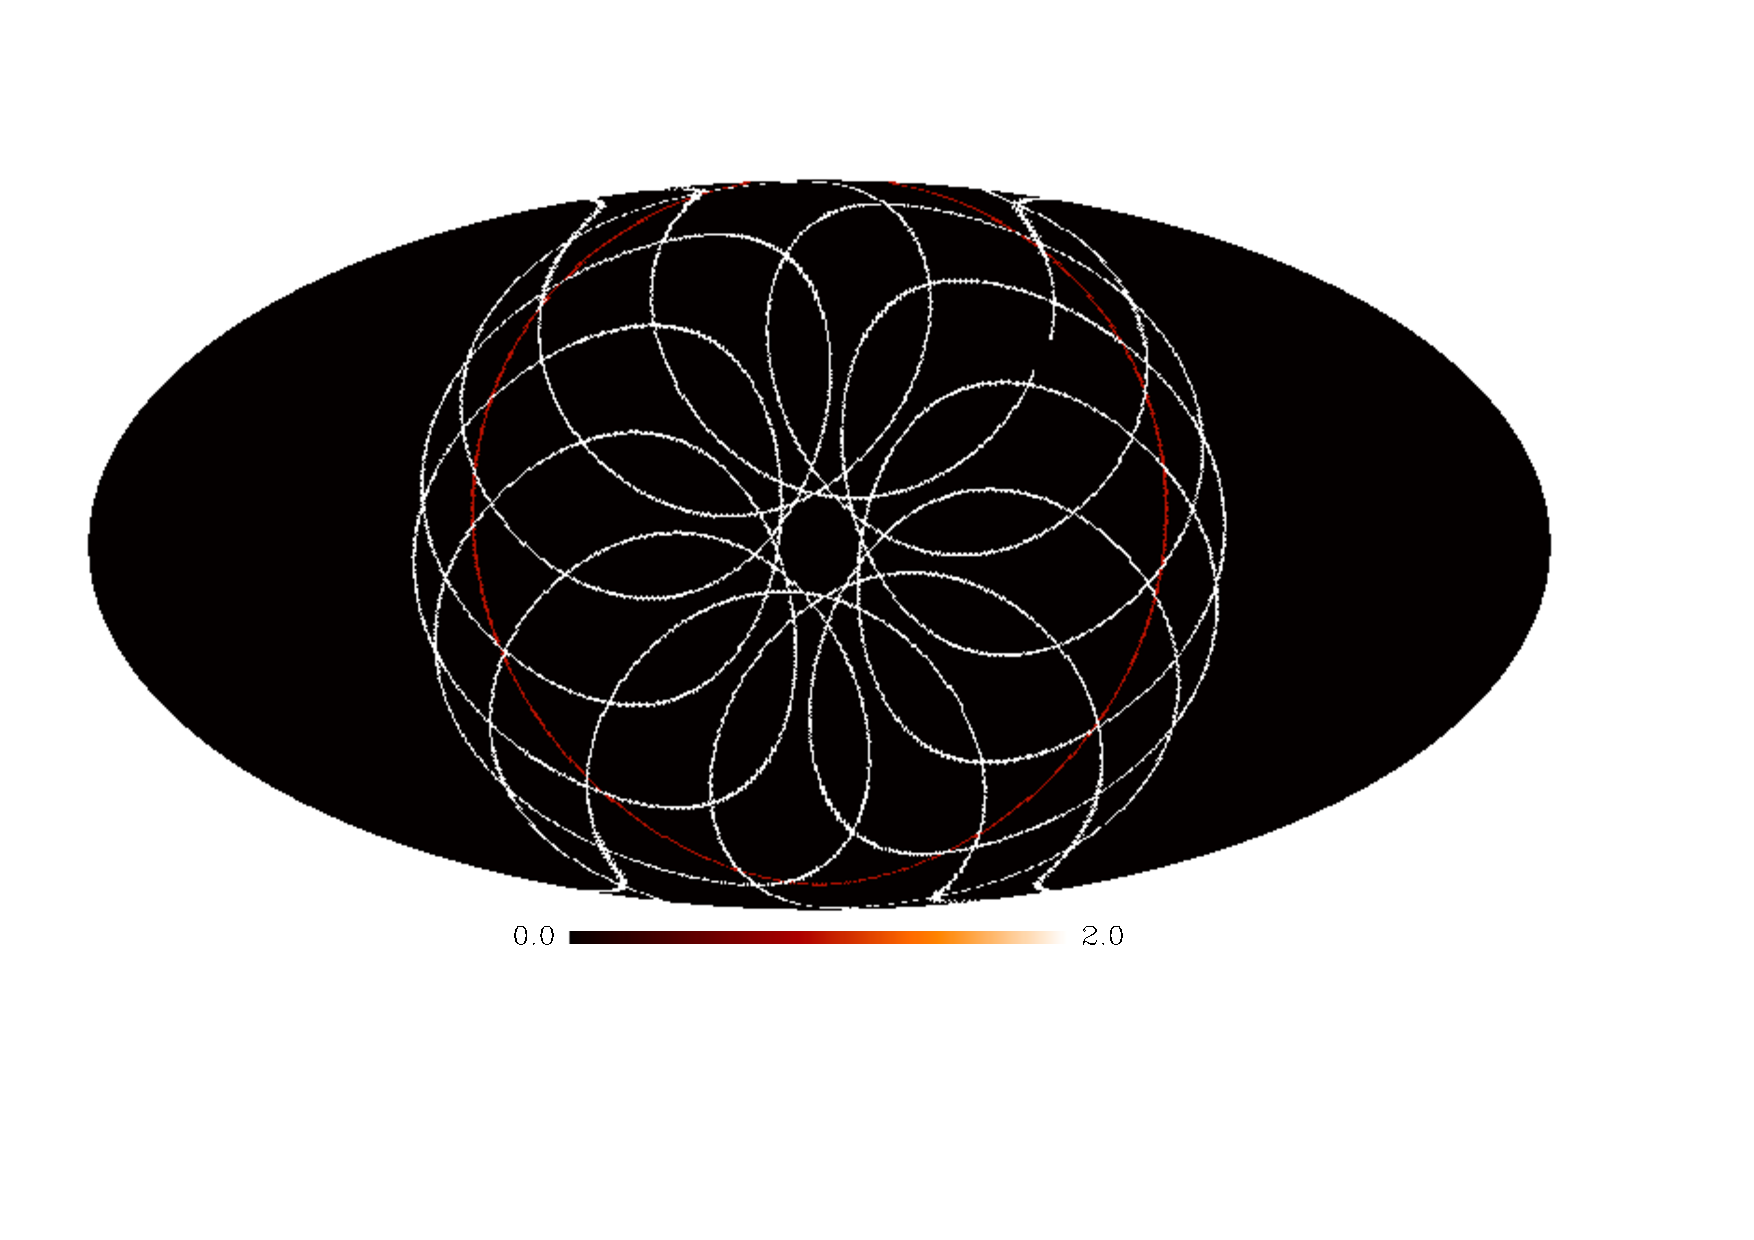
\includegraphics[clip,angle=0,width=\columnwidth]{Figures/plot_mollweide.pdf}
  \caption{White : representation of EPIC scanning strategy. Red : representation of Planck scanning strategy }
  \label{fig:strat-polsat-Planck}
\end{figure}

In the context of a CMB experiment mapping a large fraction of the sky, one should also consider the CMB dipole  with its 6.73\,mK peak to peak \citep{2015IJMPD..2430004B} converts into a \todo{XXX\,Jy} signal. The CMB dipole is a smooth gradient in the CMB temperature accross the sky. It is the result of the motion of the local group of galaxies with respect to the reference framed defined by the CMB. The CMB dipole amplitude is $\Delta T = 3.365 \pm 0.027$ mK and directed toward $(l,b) = (264.4 \degree \pm 0.3 \degree , 48.4 \degree \pm 0.5 \degree)$ in galactic coordinates \citep{1993ApJ...419....1K}. It can displace the zero level $Z$ along the circle so that a bright source would enter the non linear regime sooner than expected. This is also true for strong Galactic emission like that of Dust at frequencies above $\sim 100$\,GHz. 

\begin{figure}[h]
  \includegraphics[clip,angle=0,width=\columnwidth]{Figures/histo_galaxy_dipole.eps}
  \caption{}
  \label{fig:histo_galaxy_dipole}
\end{figure}

%Here we scan a map of the Galaxy with the two pointing strategies described earlier. In addition to the Galaxy, there is another signal that we have to take into account which is the CMB dipole. The CMB dipole is a smooth gradient in the CMB temperature accross the sky. It is the result of the motion of the local group of galaxies with respect to the reference framed defined by the CMB. The CMB dipole amplitude is $\Delta T = 3.365 \pm 0.027$ mK and directed toward $(l,b) = (264.4 \degree \pm 0.3 \degree , 48.4 \degree \pm 0.5 \degree)$ in galactic coordinates \citep{2015IJMPD..2430004B}. Like in the precedent simulations we add the template of HWP that we subtract after the signal goes through the KID model.
%
%We have seen previously that to be in a linear regime, constraints had to be put on the scanning strategy, especially on the scanning speed, and on the incoming flux. Here the scanning strategy that we use ensure that we respect the Nyquist criteria, by having a number of points per beam between 3 and 5. Plus, we can see in Fig.~\ref{fig:histo-gal-dip}, that the flux of the Galaxy and Dipole does not go higher than 20 Jy and that the two methods \rf\ and \cf\ can reconstruct it.


%% \todo{keep for global conclusion:} In conclusion, because we can not directly
%% measure the optical power from a KID, new methods were developed to monitor the
%% shift of the resononance frequency of the detector. First with the modulated
%% readout technique we can calculate four quantities : $\I$, $\Q$, $\di$,
%% $\dq$. With these quantities in hand, we can monitor the shift of the resonant
%% frequency and derive the corresponding incident power ny using the two methods
%% that were developed : \rf\ which is already successfully used in \nika\ and
%% \nika2\ (see \citep{2014A&A...569A...9C}) , and \cf\ which is an improvement
%% from \rf . In this paper, we compare these two methods in terms of linearity. To
%% do so, in the next sections we do simulations of observations by a KID and we
%% use \rf\ and \cf\ to reconstruct the signal. We then study the impact of the KID
%% non-linearity on the search for B modes polarization of the CMB.


\clearpage
\newpage

\section{Conclusion}
\label{conclusion}

\todo{Recall that we are in fact interested in the unknown difference between
  the model and the measure, not specifically its linearity that can be
  considered as a first order approximation to any differnce between an a priori
  known calibration curve}\\

\todo{aussi faire remarquer que l'eq.~(\ref{eq:eq-NL}) is linear in $\epsilon$,
  so we have further mitigation by the average of many detectors around their
  known calibration curve.}\\

This paper presents the study of KIDs systematic effects such as the non-linearity and an application to the CMB polarization. 
KIDs are a new kind of detectors based on superconducting technology that provides high sensitivity. They have been developed for the construction of NIKA and NIKA2 since 2007, which is now the first operational instrument using KIDs. One of the key asset of KIDs is their natural multiplexing capability which makes them one of the best candidates for future space mission that needs large size detector array. In this context, in a first part, we studied the response of a KID by using two methods to reconstruct the signal (\rf and \cf) and its systematic effects caracterized by its non-linearity coefficient \eps. For an incoming source consisting of a planet of 500 Jy, the dipole and a HWP, and for different scan speed, we found $\varepsilon_{rf}$ $\simeq 10^{-5}$ and $\varepsilon_{cf}$ $\simeq 10^{-7}$. The non-linearity depends on the way that we reconstruct the signal, and even if \rf can reconstruct the signal very well, \cf is better at it and generates less non-linearities. Another good point is that the modulation of the HWP does not bias the measurement by inducing large non-linearities. We have seen that in order to have less non-linearities, we need to put constraints on the scanning speed, so in a second part, we did more realistic simulations, by scanning a map of the Galaxy and dipole by using satellite pointing strategies. We found, that depending on the incoming sources, $\varepsilon_{rf}$ varies between $10^{-7}$ (Galaxy only) and $10^{-3}$ (Galaxy, dipole, HWP), and $\varepsilon_{cf}$ varies between $10^{-8}$ (Galaxy only) and $10^{-4}$ (Galaxy, dipole, HWP) (POLSAT, VOIR PB PLANCK). The results show that in a space context KIDs are capable of accurately reproducing the signal and that as in the precedent simulations \cf is slightly better than \rf.\\
The measure of CMB $B$ modes polarization is a major goal of observational cosmology, as their detection would sign the presence of primordial gravitational waves and provide a confirmation of inflation. Observations of CMB polarization demand a high control of systematics effect and in light of this, we demonstrated the capabilities of KIDs arrays to detect B modes polarization by comparing systematic effects coming from the detector and the leakage of dust temperature into polarization maps. With HEALPix, we simulated spurious signals from a map of the Galaxy and generated modified $C_{l}$. From $C_{l}^{TE}$, we calculated the coefficient ($\varepsilon'$) related to the leakage of temperature into polarization. For a tensor-to-scalar ratio (T/S) = 0.1, 0.01, 0.001 we respectively found $\varepsilon' \simeq 2.51$x$10^{-2}$, 7.95x$10^{-3}$, 2.51x$10^{-3}$. Because the leakage of temperature into polarization maps is the systematic effect that is most likely to contaminate the detection of $B$ modes , to be able to measure them, the non-linear coefficient $\varepsilon$ related to the detector must be lower than $\varepsilon'$. In all of the precedent simulations, $\varepsilon $ varried between $10^{-3}$ and $10^{-8}$, so $\varepsilon < \varepsilon'$, therefore we can say that the KID is capable of detecting $B$ mode polarization. Finally, because of the KID multiplexing ability and its capability of detecting $B$ mode polarization, we can say that KID technology is developping toward becoming one of the best candidates to space mission and study of the CMB polarization.

 
\bibliography{biblio}

%-----------------------------------------------------
\begin{acknowledgements}
NIKA standard acknowledgements + FOCUS + E.~Hivon.\\
\todo{Acknowledgement of Planck data:} Based on observations obtained with Planck
(http://www.esa.int/Planck), an ESA science mission with instruments and
contributions directly funded by ESA Member States, NASA, and Canada.
\end{acknowledgements}

\end{document}
